\documentclass{article}

\usepackage{amsmath}
\usepackage{amssymb}
\usepackage{fancybox}
\usepackage{tikz}
\usepackage{comment}


\usepackage{cite}

\usepackage{listings}
\usepackage{color}
\usepackage{hyperref}

\definecolor{mygreen}{rgb}{0,0.6,0}
\definecolor{mygray}{rgb}{0.5,0.5,0.5}
\definecolor{mymauve}{rgb}{0.58,0,0.82}

\lstset{ %
  backgroundcolor=\color{white},   % choose the background color; you must add \usepackage{color} or \usepackage{xcolor}
  basicstyle=\footnotesize,        % the size of the fonts that are used for the code
  breakatwhitespace=false,         % sets if automatic breaks should only happen at whitespace
  breaklines=true,                 % sets automatic line breaking
  captionpos=b,                    % sets the caption-position to bottom
  commentstyle=\color{mygreen},    % comment style
  % deletekeywords={...},            % if you want to delete keywords from the given language
  escapeinside={\%*}{*)},          % if you want to add LaTeX within your code
  extendedchars=true,              % lets you use non-ASCII characters; for 8-bits encodings only, does not work with UTF-8
  frame=single,                    % adds a frame around the code
  keepspaces=true,                 % keeps spaces in text, useful for keeping indentation of code (possibly needs columns=flexible)
  keywordstyle=\color{blue},       % keyword style
  language=Octave,                 % the language of the code
  % otherkeywords={*,...},           % if you want to add more keywords to the set
  numbers=left,                    % where to put the line-numbers; possible values are (none, left, right)
  numbersep=5pt,                   % how far the line-numbers are from the code
  numberstyle=\tiny\color{mygray}, % the style that is used for the line-numbers
  rulecolor=\color{black},         % if not set, the frame-color may be changed on line-breaks within not-black text (e.g. comments (green here))
  showspaces=false,                % show spaces everywhere adding particular underscores; it overrides 'showstringspaces'
  showstringspaces=false,          % underline spaces within strings only
  showtabs=false,                  % show tabs within strings adding particular underscores
  stepnumber=2,                    % the step between two line-numbers. If it's 1, each line will be numbered
  stringstyle=\color{mymauve},     % string literal style
  tabsize=2,                   % sets default   tabsize to 2 spaces
  title=\lstname                   % show the filename of files included with \lstinputlisting; also try caption instead of title
}

% \language=[Objective]{Caml}




\title{Some notes on binary search trees}
\date{\today}
\author{David M. Doolin}


\begin{document}

\maketitle

\abstract{A few notes on binary search trees and their implementations
in various programming languages. Theory and implementation details are
given equal treatment.}

\tableofcontents

\section{Introduction}


The following topics will be discussed:

\begin{itemize}

\item Differences in implementations between programming languages.
\item How best to containerize, including pure tree node, tree wrapper with
node class, abstracting keys.
\item Theory and performance.

\end{itemize}

\newcounter{sno}
\setcounter{sno}{0}
\newcommand\sno{\stepcounter{sno}$^{\thesno}$}


\section{Use of Binary Search Trees}

Online research for uses of binary testit{search} trees returns very few actual
use cases. Nearly all the writing on the topic is devoted to properties
of binary search trees (or binary trees in general), or why balancing the
tree is important. While explicit implementation of binary search trees does
not appear to be common, the data structure does appear to be commonly used
as a key-value store backing \texttt{map} and \texttt{set} structures
in various programming languages such as C++ and Java.

There is a considerable and useful amount of discussion
about binary trees in general, which is outside the scope
of this study.

One situation where both fast insertion and sorted order matter is
online sorting, where for whatever reason, incoming data needs to be
sorted for fast access requirements.



\section{Literature review}

Skiena~\cite[pp. 77, 370, 375, 589]{skiena} has a few notes.

Aho and Ullman~\cite[pp. 210]{aho:av:1992} define height and depth for nodes in a binary tree.

\begin{quote}
The height of a node n is the length of a longest path from n to
a leaf. The height of the tree is the height of the root. The depth or level of
a node n is the length of the path from the root to n.
\end{quote}

Cormen et al.~\cite{cormen:th:1990} remains a classic reference.

Rosen~\cite[pp. 757-760]{rosen} discusses three uses for binary search trees:

\begin{enumerate}
\item storing items from a list such that they can be easily found;
\item finding an object in a collection of similar objects;
\item efficiently encoding characters in a bit string.
\end{enumerate}

Sedgewick~\cite{sedgewick:r1990}.

O'Rourke~\cite{orourke:j1998}.

Manber~\cite[p. 87, Ex. 4.8]{manber:u1989} provides an interesting exercise:
show the AVL tree formed by inserting the ordered sequence $[1, 2, \ldots, 20]$.

F. Thomson Leighton discusses binary trees used in parallel computing~\cite[p. 407]{leighton:ft1992}.

\section{The Binary Search Tree}

List of relevant theorems and corollaries:

\begin{enumerate}
  \item $n$ vertices implies $n-1$ edges (Rosen~\cite[p. 752]{rosen}).
  \item Number of nodes $n$ in a complete binary tree of height $h$ is $2^{h+1} - 1$
    (Aho and Ullman~\cite[p. 257]{aho:av:1992}).
  \item A full binary tree is with $i$ internal vertices contains $n = 2i + 1$ vertices.
    (Rosen~\cite[p. 752]{rosen}).
  \item Lookup time $T$ on a binary search tree is governed by the recurrence
    $T(h) \leq T(h-1) + O(1)$ (Aho and Ullman~\cite[p. 256]{aho:av:1992}).
  \item There are at most $2^h$ leaves in a binary tree of height $h$ (Rosen~\cite[p. 754]{rosen}).
  \item Search hits in BST from $N$ random keys require $\tilde2\ln N$ (about $1.39\ln N$) compares
    on average (Sedgewick and Wayne~\cite[p. 403]{sedgewick:r2011}).
  \item Sum of heights of complete binary tree, from Manber~\cite[p. 34]{manber:u1989}.
  \item AVL tree height from Manber~\cite[p. 75]{manber:u1989}.
  \item Complete binary tree embedding on a lattice, from Manber~\cite[p. 263]{manber:u1989}.
  \item Range searching with BST in Sedgewick~\cite[p. 373]{sedgewick:r1990}.
  \item V \& H line intersection with BST from Sedgewick~\cite[p. 391]{sedgewick:r1990}.
  \item Trapezoidal locations with BST, from O'Rourke~\cite[p. 289]{orourke:j1998}.
\end{enumerate}

The theorems need to get moved to properties. Some of the above list should be
moved to a future Applications section.

\subsection{Vertex-edge relation}

\textit{Theorem: A tree with $n$ vertices has $n-1$ edges.}

Basis step: $n = 1$: a tree $T$ with 1 vertex has 0 edges.

Inductive step:

\begin{enumerate}
  \item Inductive hypothesis: a tree $T$ with $k$ vertices has $k-1$
    edges.

  \item Advance the argument: Suppose $T$ with $k+1$ vertices, and $v$ a
    leaf of $T$ with parent $w$. We want to show $k$ edges.

  \item Remove $v$ and the edge $\overline{vw}$ to produce $T'$ with $k$
    vertices. $T'$ is connected with no circuits.
  \item TODO Apply Inductive hypothesis.
  \item TODO Complete inductive step.
\end{enumerate}


\subsection{Properties and Operations}

Random definition from Aho and Ullman: \textit{branching factor}
is the maximum degree of any node in a tree (Aho and Ullman~\cite[exercise on
p. 259]{aho:av:1992}).

\begin{enumerate}
\item Operations for manipulating BSTs;
\item intrinsic properties of BSTs.
\end{enumerate}


Operations include:

\begin{itemize}
  \item Efficient insertion and deletion.
  \item depth-first search by key
  \item forward and backwards traversal from any node.
  \item breadth-first search
  \item node presence
  \item delete node
  \item Search for node successor and predecessor
  \item Maximum and minimum queries.
\end{itemize}

\section{Properties of BST}

Properties of the data structure include:

\begin{enumerate}
  \item the keys are required to posess a \textit{total order}; every key must
        be comparable to every other key.
\end{enumerate}

The keys in a BST are generally assumed to be unique, hence little guidance on
implementation which may require handling keys which are not unique. Unique keys
can be handled in two ways:

\begin{enumerate}
  \item reject the node with the duplicate key with error (or whatever);
  \item replace the existing node with new node.
\end{enumerate}

For an implementation where nodes are externally created, then inserted,
the second case might allow for updating the value associated with the existing
node with the value of the incoming node containing the duplicate key.

Non-unique keys would need to be managed with some sort of data structure at
each node. Could be interesting to implement.

Properties include:

\begin{itemize}
  \item height
  \item depth
  \item maximum key
  \item minimum key
  \item size
  \item diameter
  \item class (full, perfect, complete, balanced, etc.)
\end{itemize}

Node properties include:

\begin{itemize}
  \item visited and unvisited
  \item has unvisited children
\end{itemize}

\subsection{Structural uniqueness of binary search tree}

Hypothesis: each different preorder traverse of a binary search
tree corresponds to a unique binary search tree. In other words,
every structurally unique binary search
tree has a unique preorder traverse.

I think this is true.

If it is true, it provides an easy to compare binary
search trees, just compare the result of an inorder
traverse, or define a function which compare nodes in
parallel during an inorder traverse of each.

Keys are assumed to be unique.

\subsection{Height}

\subsection{Depth}

\subsection{Size}

\subsection{Diameter}

\subsection{Classification}

Binary search trees may be classified according to the
arrangement of the leaves and internal nodes.
Binary search tree classifications include
full, perfect, complete, balanced, unbalanced, and degenerate.

First, how these classifications are defined in the literature is
worth some discussion, as different authors define trees in slightly
different ways. For example, Aho and Ullman define full and complete
trees as the same~\cite[p. 257]{aho:av:1992}, whereas Cormen
et al.~\cite[p. 1178]{cormen:th2009} distinguish between full and
complete binary trees.

The definitions which follow will be used consistently through this
work. The reader is free, of course, to take issue and use definitions
more to his or her preference.

\begin{itemize}
  \item Full: A rooted tree is called an m-ary tree if every internal
    vertex has no more than m children. The tree is called a full m-ary
    tree if every internal vertex has exactly m children. An m-ary tree
    with m = 2 is called a binary tree.~\cite[p. 748]{rosen} Also see
    Cormen et al.~\cite[p. 1178]{cormen:th2009}.

  \item Complete: A binary tree is complete when each child of the root node,
    left and right, is a complete subtree (Aho and Ullman). Cormen et al.\
    define complete as all leaves having the same depth with all nodes having
    having degree 2, that is, 2 children. This is equivalent to saying all
    internal nodes are full~\cite[p. 1179]{cormen:th2009}).
\end{itemize}

\subsection{Maximum and minimum keys}

\setcounter{sno}{0}

\sno Maximum and minimum elements of binary search trees are probably the easiest
algorithms to both understand and implement. \sno The maximum is the right-most
node, the minimum the left-most, finding either means traversing the tree
to the appropriate leaf, and returning that node which has no children.

\sno The maximum function written in Ruby is particularly elegant,
we take advantage of Ruby's safe navigation operator {\tt \&}:

\lstset{language={Ruby}}
\begin{lstlisting}[frame=none]
def maximum
  right&.maximum || self
end
\end{lstlisting}


\section{Building a binary search tree}

\subsection{Collisions or duplicate values}


None the preceding references explicitly discuss collisions.

\begin{itemize}
\item The duplicate key can be added to the tree, either silently or with a warning.
\item The duplicate key is not added to the tree, either silently or with a warning.

\item In Ruby, does replacing a node in a tree leak memory, or will the deleted node
get garbage collected? How about Python?

\item How to delete in c/c++ such that memory isn't leaked? This should be easier,
call delete after the node is orphaned.
\end{itemize}



\section{Operating on the BST}

Abstract data structures such as binary search trees support a standard
set of operations including insertion, deletion, search, etc. A closer look
at each of these operations follows.

\subsection{Least common ancestor}

The \textit{least common ancestor} (LCA) of two nodes $v$ and $w$ in a tree $T$ is the
lowest or deepest node which has $v$ and $w$ as descendants of itself, and where
each node is defined as a descendant of itself. The LCA is the shared ancestor located
farthest from the root of the tree $T$. Consider the following 3 node binary search tree.

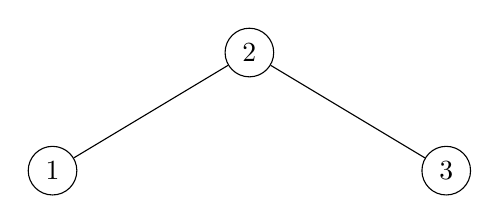
\begin{tikzpicture}[level/.style={sibling distance=50mm/#1}]
  \node [circle,draw] (z){$2$}
    child {node [circle,draw] (a) {$1$}}
    child {node [circle,draw] (j) {$3$}
  };
\end{tikzpicture}

We have the following cases:

\begin{enumerate}
  \item 1 is the LCA of 1.
  \item 2 is the LCA of 2.
  \item 3 is the LCA of 3.
  \item 2 is the LCA of 1 and 3.
  \item 2 is the LCA of 2 and 3.
  \item 2 is the LCA of 1 and 2.
\end{enumerate}

At least two algorithms may be employed to determine LCA. The first algorithm makes
two passes through $T$ to find a path from the root to the node. The second makes a
single pass through $T$, once down each branch. For the first algorithm, implementing
a path to node method is not difficult as it uses the same mechanics as the find method.

\lstset{language={Ruby}}
\begin{lstlisting}[frame=single,title=Two pass algorithm for LCA.]
def least_common_ancestor(key1, key2)
  (path(key1, []) & path(key2, [])).last
end

def path_to_node(key, collector)
  node = find(key) { |n| collector << n.key }
  raise KeyNotFoundError if node.nil?

  collector
end
\end{lstlisting}


\subsubsection{Error conditions}

The LCA algorithms fails if either node is not present in $T$. Handling this
condition is implementation dependent.


\subsection{Depth-first traverse}

\lstset{language={Ruby}}
\begin{lstlisting}[frame=single,title=Traverse the tree from the bottom up.]
def postorder_iterate
  return unless root

  current = find_unvisited_leaf_node root
  yield current

  while current.has_parent?
    current = find_unvisited_leaf_node current.parent
    yield current
  end
end
\end{lstlisting}

\lstset{language={Ruby}}
\begin{lstlisting}[frame=single,title=Find the deepest leftmost unvisited node relative to current.]
def find_unvisited_leaf_node current
  while current.has_unvisited_children?
    if current.left&.unvisited?
      current = current.left
    elsif current.right&.unvisited?
      current = current.right
    end
  end
  current.visit
end
\end{lstlisting}

\subsection{Successor and predecessor}

\setcounter{sno}{0}

\sno For an ordered list of values $x_i \in [x_0, x_1,\ldots,x_k]$, the successor of
$x_i$ is $x_{i+1}$, the predecessor $x_{i-1}$.

\sno Cormen et al.~\cite[p. 248-249]{cormen:th:1990} provide a succinct algorithm for
determining the successor given each node is linked to its parent.

\sno A decision has to made regarding the definition of minimum and maximum
elements in the tree. \sno The choices are having the relevant successor or
predecessors of such elements either be nil or be the node. \sno For this implementation,
maximum nodes are their own successors and minimum nodes are their
own predecessors.

\sno Here's an implementation in Python. \sno The nodes do not have a parent
pointer, so the parent must be passed along the recursion, along with
the correct predecessor.

\lstset{language={Python}}
\begin{lstlisting}[frame=single]
def get_predecessor(self, node, parent, predecessor):
    if parent.right == self:
        predecessor = parent

    if node.key == self.key:
        if self.left is not None:
            return self.left.minimum()
    else:
        return predecessor

    if node.key < self.key:
        if self.left is not None:
            return self.left.get_predecessor(node, self, predecessor)
    else:
        if self.right is not None:
            return self.right.get_predecessor(node, self, predecessor)

def predecessor(self, node):
    return get_predecessor(node, self, node)
\end{lstlisting}

\sno Implementing {\tt successor} is easy, use right for left, and find the
maximum where predecessor finds the minimum.

\subsection{Unvisit}

An \method{Unvisit} method needs to be implemented to ensure that once the
necessity for evaluating nodes for visited state has passed, all
the nodes in the tree can be reset to \attribute{visited = false}, allowing
future operations to proceed correctly. Implementation is easy,
simply pass a callback to any of the tree traversal functions which
sets \attribute{visited = false}.


\section{Properties of nodes}

Trees and nodes aren't the same thing, there is a logical separation.
That said, the behavior of the tree sometimes depends on the state of the
node.

\subsection{Visited and unvisited state}

When we visit a node during a walk or traverse of a tree, it might be
useful to mark whether the node has been visited. This is important, for
example, when performing depth-first searching, where the ``cursor'' has
to backtrack. The following methods help make the implementation easy
to understand:

\begin{itemize}
  \item \method{Visit} sets the node attribute \attribute{visited = true}.
  \item \method{Is\_Visited} (or \method{Visited?}) replies with the boolean
    state of the node, true when the \attribute{visited} is set.
  \item \method{Is\_Unvisited} (or \method{Unvisited?} is the default state
      of each node.
\end{itemize}

\subsubsection{Test cases for \method{Visited?} and \method{Unvisited?}}

Testing is almost superfluous. For TDD, the tests can be set up
to verify that setting and unsetting the visited state is correctly
performed. Later, these tests could be removed and the visited and
unvisited helper methods moved to private methods.

\subsection{\method{has\_unvisited\_children?}}

\lstset{language={Ruby}}
\begin{lstlisting}[frame=single,title=Helper methods for determining child's status.]
def unvisited?
  !visited
end

def has_unvisited_children?
  return false unless has_children?
  left&.unvisited? || right&.unvisited? ? true : false
end
\end{lstlisting}

\section{Breadth-first traversal}

Breadth-first traveral can be used for searching, for determining whether a key exists,
or for writing out the tree in flat format with rows and pointers.

For persistence, we have the following:

\begin{itemize}
\item At each node we can store pointers to each child.
\item We can store the start and the stop of each row separately.
\item We can store an array of arrays, where each of the arrays is
      one level of the tree.
\end{itemize}

[
 [root],
 [ root.left, root.right],
 [...]
]

Can all the pointers be stored in one pass, then process in a second pass,
or can the nodes be processes as the breadth-first traverse proceeds?


\section{Containerizing}

\subsection{Tree/Node interaction}

Trees are abstract data types. This makes trees easy to reason about.
Implementing a tree requires dealing with a number of subtle issues.
Since Trees are usually described in terms of the Nodes comprising
the Tree, some thought about differentiating Trees and Nodes is in order.

\subsubsection{Implicit structure}

Given some class, record, structure or whatever language feature which contains
data and supports function invocation, adding left and right pointers,
appropriate comparators, and insert and find methods suffices to provide
dictionary capability to the given language feature. However, trees require a
root, and managing this root increases the complexity whatever application
system requires the data sorted into the tree. Provision needs to be made for
the root changing, or even being deleted.

\subsubsection{Tree container}

Another way to implement trees is to create a tree container which implements
insert, search, etc. The implementation provided by the tree container could
implement the functionality itself, or call an implementation provided by
the node element.

\subsubsection{The BST Node}

By definition, each node in a binary search tree contains a left child and
a right child, either or both of which may be nil.

Some operations on binary search trees, such as {\tt delete}, require
the node's parent as well as its children. The parent to any node can also
be stored as a reference or pointer, or the parent can be determined at
runtime.

Storing parent pointers is easy. When inserting a node as a child, set that
node's parent pointer to the inserting node.

Determining parent pointers at runtime is not conceptually much more difficult:
keep track of the parent at each node by passing the current node to the
recursive calls. Two disadvantages of this include longer argument lists
for recursive calls, and either returning both node and parent when necessary.
For languages which do not allow multiple return values, one of the arguments
will have to capture the state change for access by the calling method.
In theory, this is straightforward. From an engineering standpoint, requiring
both a return value and an argument state change violates the principle of
least astonishment.

Passing both node and parent back through the argument list is a pretty good
case for adding the parent node directly to the Node data structure.


\subsection{C++ templating}

\subsection{C struct inclusion}

\paragraph{private headers}

\subsection{Ruby module inclusion}

It's not difficult to encode binary search tree capability into a Ruby module.
The module provides all the necessary instance binary search tree methods, and
raises errors when necessary overriding has not been implemented in the
including class.

The usual caveats about instance variables referenced in modules applies,
particularly that the including class must define the key for the tree.

\section{AVL tree}

AVL trees are a type of binary search tree which maintains height balance
on insert operations by \textit{retracing} the insertion path of the node,
and performing \textit{node rotation} at every node in the retrace path
which became unbalanced on the insert. AVL trees are not that technically
difficult to implement, but there are a few tedious details requiring
precise attention. Some factors to consider:

\begin{enumerate}
  \item Where the retracing is implemented depends on how the tree and
    node data structures are implemented. Because the root node may change
    as a result of rotation, the Tree data structure will have to have a way
    of ensuring the current root is valid.
  \item Retracing can be done from the tree, or as part of the node capability.
  \item Rotations ultimately decompose into two cases. The first case is moving
    a left (right) child into its parent's position, the other case is swapping a right (left)
    child for its parent, where both cases require ensuring all relevant pointers
    are updated accordingly.
\end{enumerate}

We'll work our way backwards through the above list, starting with a detailed
discussion of rotation, which is the fun part everyone wants to do anyway.

\subsection{Rotation}

There are plenty of references, web sites, Youtube videos and whatnot
where AVL rotation is explained in detail. None of them are wrong, but
most go into extraneous detail far too quickly, presenting situations
which will be hard to visualize during implementation, and possibly
difficult to construct for testing. It turns out, as claimed above,
that rotations are fundamentally about parent/child repositioning
while ensuring all the relevant pointers are updated accordingly.

Ironically, it's easier to motivate rotations using 3 nodes instead
of two nodes. The idea is putting a binary search tree back into
balance, and by definition, and AVL tree of size 2 is balanced.
So we need 3 nodes to see what the problem is, and how to solve it.

Three nodes results in 5 different binary search trees. We may discard
the balanced tree from our conversation immediately, leaving the other
4 trees out of balance, by definition. Of these 4 trees, we can use
symmetry to dispose of all the remaining trees with nodes right (or left)
leaving two cases to consider. While both cases are ``skew'' trees
(all the nodes have one and only one child), it's useful to note
that Case 1 has left children only, and Case 2 has a left child then
a right child. (Conversely, right children only, and right then
left child). We'll call Case 1 a \textit{left chain} and Case 2 a
\textit{left knee}.

FIGURES HERE.

\subsubsection{Left chain}

Suppose in the left chain we have a root keyed 17, and child left
7, then 2. For balance, we want the new root to be 7, with right 17
and left 2.

It's helpful here to distinguish between the root of the tree, and a
some local \textit{rotation root}. In this base case, the tree root
and the rotation root are the same node. In the general case, the
tree root and rotation root will be different, and we're going to
lean on our rapidly developing data structures intuition to keep the
context straight.

Continuing, the node keyed 17 is chosen as the \textit{rotation root}.
The node 7 we'll call the \textit{pivot}. Implementing this rotation
to balance the tree requires:

\begin{enumerate}
  \item Save the parent pointer of the rotation root (nil in this case).
  \item Move the node 17 to 7's right child, updating 17's parent pointer.
  \item Set 7's parent pointer to the saved value.
\end{enumerate}

\subsubsection{Left knee}

In the left knee, let's have our root 17, with left 7, and 7's right
child 11. In this case, we want 11 to be the root, with 7 as left
child and 17 as right child. Simply moving 7 into the tree root
position won't work, it will violate the binary search tree definition.
And besides, we can't put 17 on 7's right, 11 is already there.
Instead, what we do first is rotate to make a chain, then rotate
our new chain into balance.

And it turns out making a chain from knee is easy: choose the middle
node as the rotation root, the right child as the pivot, and rotate
counterclockwise. Now the tree looks like $7 \leftarrow 11\leftarrow 17$, and we
already know how to balance a left chain.

Above, we threw away the right side of the tree by invoking symmetry.
By invoking symmetry again, we get the right side of the tree back,
swapping `left' for `right' and `right' for `left.'


\paragraph{Why the base cases are important}
Invoking the property of the AVL tree, inserting a node triggers retracing,
which may result in rotations to rebalance.  Given random keys, it's
at least average behavior (I claim!) that an AVL tree is going to rebalance after
inserting the third node. The chain and knee situations above must be handled
correctly to proceed with general implementation of AVL tree.


\subsection{Rotation beyond the base cases}

The above is all well and good for trees of size 3, which is to say, useless.
Child nodes are subtrees with possibly very large subtrees of their own,
and inserting a node which travels all the way to a leaf at the bottom
of the tree might trigger rotational adjustment all the way back to the
root of tree. This is less of a problem than it would seem: the base
case implementation requires one additional concept, that of a
\textit{swing node} which changes its parent pointer from the pivot to
the pivot's previous child position on the rotation root. While that
seems complicated, and may not be exactly trivial, it's a relatively
straightforward extension of the base case rotation.

That is to say, our new friends chain and knee still control the structure
of the rotation.


\subsection{Retracing}

Retracing is the operation of iterating from the inserted
node up the tree, possibly (always?) to root, checking
the balance at each node and rebalancing if necessary.
Rebalancing is simply applying the correct rotations,
either the simple right or left, or the double rotations
as the case may be.

Retracing has three challenges:

\begin{enumerate}
  \item Determining or maintaining balance factor at each parent,
  \item distinguishing between ``chain'' and ``knee'' rotations, and
  \item Ensuring the relationship between the rotation root, the pivot
    and the rotation root's parent is correct.
\end{enumerate}

If the weight or ``balance factor'' is maintained at each node, it must be
adjusted during the rebalancing process. If balance factor isn't maintained at
each node, the height of each subtree at each node will be required, which is
expensive.

Some rotations will move the rotation root to a child position, which
requires resetting its parent to the pivot, and ensuring that the
pivot and the rotation root's previous parent are linked.

\paragraph{Chain versus knee rotations}

\subsection{Implementation design}

Assuming we want to maintain an accurate node pointer for the root of the tree,
at the highest level, retracing needs to be controlled by the same data
structure in charge of the root node. In a node/tree situation, retracing
belongs to the tree. Since retracing is performed bottom up from the
inserted node, the tree data structure needs to keep a reference to
the inserted node, which requires insertion to be controlled by the
tree as well.

One critical part for correctly implementing an AVL tree's knowledge of
it's height balance at every node. For example, the reference implementation
displayed on Wikipedia manages height balance by adjusting the
\textit{balance factor} on every rotation, and during retracing. That is,
balance factors are adjusted in two places. The reader is excused if
he or she finds splitting the work confusing, it is confusing. If possible,
balance factors should be updated in one place.

\section{Red-black tree}

The Red black-tree appears to have a reputation of being both ``the last word''
in binary search trees (outside of specialist literature) and a fearsome
reputation among programmers in practice. One might speculate this reputation
is founded on the red-black tree being about as complicated as any particular
undergraduate data structure. For whatever reason, it seems to come up on a
regular basis in those discussions on what programmers should or should not be
expected to be proficient in for job interviews. One camp holds that basic data
structures (i.e., reb-black trees, etc.) should be at a programmer's
fingertips, the other that book learning from 30 years ago is hardly relevant
for shipping code daily.

But we don't case about such things. Our interest is in the thing itself.


\section{Persistence}

Here are some ways to store the structure in text format:

\begin{enumerate}
\item Write to nested json. This requires writing out from the top
down. Should be able to do this by converting to hash, then
writing to json. Reading in is the reverse. How to convert a
hash to a binary tree? Maybe this is where to use combinator.

\item CSV: does this require top down, or can it be done by traversing?
Does it require a parent pointer?

\item Yaml: how are references handled?
\end{enumerate}


\section{Summary}


\subsection{Links}

\begin{itemize}
\item \href{http://aofa.cs.princeton.edu/60trees/}{http://aofa.cs.princeton.edu/60trees/}
\item \href{https://en.m.wikipedia.org/wiki/Stern-Brocot\_tree}{https://en.m.wikipedia.org/wiki/Stern-Brocot\_tree}
\item \href{https://en.m.wikipedia.org/wiki/Day-Stout-Warren\_algorithm}{%
https://en.m.wikipedia.org/wiki/Day-Stout-Warren\_algorithm}
\item \href{https://en.m.wikipedia.org/wiki/Tango\_tree}{https://en.m.wikipedia.org/wiki/Tango\_tree}
\item \href{https://en.wikipedia.org/wiki/Geometry\_of\_binary\_search\_trees}{%
https://en.wikipedia.org/wiki/Geometry\_of\_binary\_search\_trees}
\end{itemize}


% \section{References}

\bibliography{references}{}
\bibliographystyle{plain}


\appendix

\section{Implementation}

Implementing binary search trees is superficially very easy. Nevertheless,
a number of design decisions must be made. There is also the challenge of
implementing any algorithm well.

One of the gaols of this exercise is to implement binary search trees in multiple
programming languages, including languages with which the author is either
minimally competent, or unfamiliar. Expertise is acquired by hard work and
learning from mistakes, and the faster those mistakes are exposed, the
faster expertise may be approached.

In general, the various implementations were developed following this
pattern:

\begin{enumerate}
\item Install a minimal development environment for each language, focusing on
application structure where testing is supported. Languages without a workable
testing framework have not (and likely will not) be used.
\item Implement a simple, working binary search tree using test driven development.
The initial implementation will be massively over-tested, a consequence of
test-driving each method's implementation.
\item The test suite now provides regression protection, allowing simplistic
method implementations to be iteratively refined, with the goal being production-quality
code indistinguishable from professionally and idiomatically implemented code
for each programming language. This refinement may take more than a single iteration.
\end{enumerate}

For example, the {\tt is\_bst} function implemented in Java used a helper
method on the first iteration. A better way to implement might be to pass
a closure to a generic {\tt in\_order\_traverse} function, similar to how
the Ruby {\tt bst?} implementation works.

\subsection{Handling null/NULL/nil/etc}

Key to any BST algorithm is the notion that leaf nodes are represented
by empty leaf nodes. Empty nodes have no key, no value, and need not be
instantiated. They must, however, be denoted in some way, which is
usually accomplished by setting the relevant child pointers (left and
right) to whatever the programming language regards as a ``non-value.''
For example, in C this is {\tt NULL}, in C++ {\tt nullptr}, in Python {\tt None}.

(It would be possible to define a global external node.)

\subsection{Testing}

Two ways of arranging tests include:
\begin{enumerate}
\item Group tests by method or function, ensuring a number of different
trees pass the method being tested.
\item Group tests by the tree, ensuring each operation on that particular tree
executes correctly.
\end{enumerate}

Traditionally, in Test-Driven Design (TDD), a method test is created with a simple example.
The method is then implemented as simply as possible to ensure the example passes.
More complex examples are created, and the method's implementation modified as necessary
to ensure tests pass. For example, when implementing {\tt insert}, it makes sense
to write a test specification to check the a node is correctly inserted into an
empty tree to form the root, another test specification to ensure the inserting
to the left of root works correctly, to the right of root, and so on. However,
when implementing, say, {\tt size}, the same sort of procedure follows in test-driven
development: test the null case, then the cases 1 node, 2 nodes, etc.

Once the data structure is implemented, this TDD process results in a large number
of redundant tests.

Grouping tests by data structure examples puts a much larger burden on TDD,
but provides a different perspective. These tests may be more effective once an
initial implementation is created. Then, pathological data structures can be
created and tested in detail.


A binary search tree using first 10 primes for keys:

%\ovalbox{%
  \begin{tikzpicture}[level/.style={sibling distance=50mm/#1}]
  \node [circle,draw] (z){$17$}
    child {node [circle,draw] (a) {$5$}
      child {node [circle,draw] (b) {$3$}
        child {node [circle, draw] (c) {$2$}}
        child {node (ca) {}}
      }
      child {node [circle,draw] (g) {$7$}
        child {node (ga) {}}
        child {node [circle,draw] (gb) {$11$}
          child {node {}}
          child {node [circle,draw] (gc) {$13$}}
        }
      }
    }
    child {node [circle,draw] (j) {$23$}
      child {node [circle,draw] (k) {$19$}}
    child {node [circle,draw] (l) {$29$}}
  };
\end{tikzpicture}
%}

This tree contains a pathological subtree rooted at the node with key 7.

\subsubsection{Insert}



\subsubsection{Collect}

Test driving may induce more tests than are strictly necessary.

\begin{enumerate}
\item Single node
\item 2 node tree right
\item 2 node tree left
\item arbitrary tree
\end{enumerate}

\subsection{Search}

Here is the algorithm to find a node in a binary search tree using the key:

\lstset{language={Python}}
\begin{lstlisting}[frame=single]

def search(self, key):
    if key == self.key:
        return self

    if key < self.key:
        if self.left is not None:
            self.left.search(key)
    else:
        if self.right is not None:
            self.right.search(key)
\end{lstlisting}

\subsubsection{Testing search}

Test cases:
\begin{enumerate}
\item finds nil with an empty tree
\item finds a node in a single node tree
\item finds the left child and right child in two node trees
\item find leaf node in tree with height greater than 1
\item finds nil when key is not in the tree
\end{enumerate}

\subsubsection{Pre- and post-order traversing}

Pre- and post-order traversing are useful for binary trees in general:

\paragraph{Pre-order traverse}

Pre-order traverse is also known as top-down traverse as the the nodes
are dereferenced from the root (pretend the tree is upside down) going
down into the tree. Pre-order traverse is good for:

\begin{enumerate}
  \item Serialization of binary search tree.
    Write node data out
    as the tree would rebuild in insertion order when read the data back in.
  \item Visually displaying a tree structure can be done with a pre-order traverse.
    Indentation would have to be handled in some way.
  \item creating pre-order parse tree for binary operations such as arithmetic
    expressed in Lisp, Scheme, etc.
  \item Useful for duplicating tree in single pass.
\end{enumerate}

\paragraph{Post-order-traverser}

Post-order traverse is also known as bottom-up traverse as the nodes
are dereferenced from the leaf nodes towards the top (root) of the
tree. Post-order traverse is good for:

\begin{enumerate}
  \item useful for freeing memory or otherwise releasing
    nodes from a tree without orphaning nodes.
  \item creating a post-order expression tree for parsing binary operations
    in post fix languages such as Postscript or Forth.
\end{enumerate}

\subsubsection{Delete}

Delete depends on search, so that will need to be implemented everywhere first.

There are three cases for the node to delete:

\begin{enumerate}
\item node has no children
\item node has one child
\item node has two children
\end{enumerate}

Other functions which are helpful for implementing delete correctly
are bst?, depth and size. These functions can all be used in the testing
code.

Write out a plan for implementing delete in java, python, c++ and lua,

\begin{itemize}
  \item including tree/node interaction, list of trees to work with,
  \item implementations for search, size, depth, and bst?
  \item algorithm writeup in bst doc, etc.
  \item After implementing and writeup, compare with clr.
\end{itemize}

Cormen et al.~\cite[p. 253]{cormen:th:1990} provide an implementation of
delete at the tree level. Advantages of this algorithm include explicit root node
deletion, and approximately retaining the tree's balance by using the deleted
node's successor.

However, it assumes that the node to delete is
given (rather than providing a key and searching for the node), and that
each node other than the root node has a link to its parent node.
Also, copying data such as the kay and whatever value(s) are associated
with the node is required. The number if {\tt if} statements also make
the logic difficult to see-at-a-glance.

\lstset{language={Python}}
\begin{lstlisting}[frame=single]
# Python implementation of delete, from CLR p. 253
def delete(T, z):
  if z.left is None or z.right is None:
      y = z
  else:
      y = z.successor(z)

  if y.left is not None:
      x = y.left
  else:
      x = y.right

  if x is not None:
      x.p = y.p # p is link to parent node

  if y.p is None:
      T.root = x
  else:
      if y == y.p.left:
          y.p.left = x
      else:
          y.p.right = x

  if y != z:
      z.key = y.key

  return y
\end{lstlisting}

Note that the returned node ({\tt y}) may or may not be the node
which was deleted. When the node to delete has two children, the
attributes of its successor node are copied into that node, and the
successor node is returned. While there is no impact at run time,
and copying attributes is arguably less complex than managing links
if moving a successor node, test cases must account for the discrepancy
in assertions. That is, removing a leaf node will return that leaf node,
for which an assertion may be written.

Here is an alternate delete algorithm in given in Ruby,
where the key provided instead of the node.
It does not require nodes to have parent links, the
parent is found along with the node. A disadvantage of
this scheme is dealing with a deleted root node. Any
enclosing tree container will have to update the
root node externally to this algorithm. Another, less
obvious disadvantage is this algorithm won't improve
the balance of the tree.

\lstset{language={Ruby}}
\begin{lstlisting}[frame=single]
def delete key, parent = nil
  node_to_delete, parent = search_with_parent key, parent
  left = node_to_delete.left
  right = node_to_delete.right

  if parent&.right == node_to_delete
    parent&.right = right
    right.insert left unless left.nil?
  else
    parent&.left = left
    left.insert right unless right.nil?
  end

  node_to_delete.left = node_to_delete.right = nil
  node_to_delete
end
\end{lstlisting}



Test cases:
\begin{enumerate}
\item deletes nil with an empty tree
\item deletes a node in a single node tree
\item deletes the left child and right child in two node trees
\item deletes leaf node in tree with height greater than 1
\item deletes nil when key is not in the tree
\item deletes the entire tree node-by-node
\item deleted node has key, left and right set to nil
\end{enumerate}

Yet another delete algorithm comes from CLRS~\cite{clrs}, with the following
cases:

\begin{enumerate}
  \item \textbf{Node z has no left child}: Replace z with it's right child
    which may or may not be nil.
  \item \textbf{Node z has left child but no right child}: Replace z with
    its left child.
  \item \textbf{Node z has 2 children where right child is successor}: 1.
    Replace z with successor; 2. Update sucessor left to point to z's left;
    3. Update z's left parent to point to z.
  \item \textbf{Node z has 2 children where right child is not successor}:
    1. Replace successor (y) with it's own right child; 2. Set y's right to
    z's right; 3. Set y's right parent to y; 4. Proceed with 3 above using
    z's right child successor.
\end{enumerate}


\subsubsection{AVL testing}

Some links for AVL trees:

\begin{itemize}
\item  \href{http://adtinfo.org/libavl.html/Step-3-in-AVL-Insertion.html}{%
http://adtinfo.org/libavl.html/Step-3-in-AVL-Insertion.html}
\item \href{http://eniac.cs.qc.cuny.edu/andrew/csci700-11/lecture7.pdf}{%
http://eniac.cs.qc.cuny.edu/andrew/csci700-11/lecture7.pdf}
\item \href{http://software.ucv.ro/~mburicea/lab6ASD.pdf}{%
http://software.ucv.ro/~mburicea/lab6ASD.pdf}
\end{itemize}

\paragraph{Insert}

\begin{itemize}
\item Draw out the cases requiring rotations. This will include 3, 4, 5, and 6
node examples, but probably no more than 6, possibly no more than 5.
\item Create a number of nodes.
\item Build the tree in sorted order starting with the smallest node.
This will build out the tree from the left, performing right, or ccw, rotations.
\item As each node is inserted, check the size, weight, balance and which node is currently the root of the tree.
\item Write an expectation for the rotate\_ccw method to ensure it's called the correct number of times.
\end{itemize}

Repeat this using the same list in decreasing order to build the tree from the
right.

Repeat inserting the keys in sorted order so the avl operation maintains
balance. Write an expectation to ensure no rotations are performed.


\paragraph{Delete}

Do something similar as above, check
rotations and balance after deletion.


\subsubsection{RB testing}

Some links for RB trees:

\begin{itemize}
\item \href{http://eniac.cs.qc.cuny.edu/andrew/csci700-11/lecture8.pdf}{%
http://eniac.cs.qc.cuny.edu/andrew/csci700-11/lecture8.pdf}
\end{itemize}

\subsection{Language listings}

\lstset{language=[Objective]{Caml}}
\begin{lstlisting}[frame=single]  % Start your code-block

open OUnit2;;

let test1 test_ctxt = assert_equal "x" (Foo.unity "x");;
let test2 test_ctxt = assert_equal 100 (Foo.unity 100);;

(* Name the test cases and group them together *)
let suite =
"suite">:::
 ["test1">:: test1;
  "test2">:: test2]
;;

let () =
  run_test_tt_main suite
;;
\end{lstlisting}

To say a child is left or right depends upon who's looking at who.
Are you looking at the tree? Or is the tree looking at you?

\end{document}
